%\documentclass[brudnopis]{xmgr}
% Jeśli nowe rozdziały mają się zaczynać na stronach
% nieparzystych:
\documentclass[openright]{xmgr}

%\defaultfontfeatures{Scale=MatchLowercase}
%\setmainfont[Numbers=OldStyle,Ligatures=TeX]{Minion Pro}
%\setsansfont[Numbers=OldStyle,Ligatures=TeX]{Myriad Pro}
% for fontspec version < 2.0
\setmainfont[Numbers=OldStyle,Mapping=tex-text]{Minion Pro}
\setsansfont[Numbers=OldStyle,Mapping=tex-text]{Myriad Pro}
%\setmonofont[Scale=0.75]{Monaco}

% Opcjonalnie identyfikator dokumentu
% drukowany tylko z włączoną opcją 'brudnopis':
\wersja   {wersja wstępna [\ymdtoday]}

\author   {Kamil Pek}
\nralbumu {231\,050}
\email    {kpek@sigma.ug.edu.pl}

\title    {TrainCMS --- system zarządzania treścią witryny internetowej}
\date     {2017}
\miejsce  {Gdańsk}

\opiekun  {dr W. Bzyl}

% dodatkowe polecenia
%\renewcommand{\filename}[1]{\texttt{#1}}
%\definecolor{stress}{cmyk}{0,1,0.13,0} % RubineRed
%\definecolor{topic}{cmyk}{0.98,0.13,0,0.43} % MidnightBlue

\usepackage{minted}
\renewcommand{\listoflistingscaption}{Spis kodów źródłowych}
\usepackage{listings}
\renewcommand{\lstlistlistingname}{Spis kodów źródłowych}

\lstdefinelanguage{bashes}{%
  language = bash,
  morekeywords = {rails, generate, uploader, sudo, apt-get},
}

\lstdefinelanguage{ruby2}{%
  language = ruby,
  morekeywords = {require, @import, include, process, render },
}

\lstset{morekeywords={include}}

\definecolor{bluekeywords}{rgb}{0.13,0.13,1}
\definecolor{greencomments}{rgb}{0,0.5,0}
\definecolor{redstrings}{rgb}{0.9,0,0}
\lstset{ %
captionpos=b,
frame=lines,
showspaces=false,
showtabs=false,
breaklines=true,
showstringspaces=false,
breakatwhitespace=true,
escapeinside={(*@}{@*)},
commentstyle=\color{greencomments},
keywordstyle=\color{bluekeywords},
stringstyle=\color{redstrings},
basicstyle=\ttfamily\small,
}

\lstset{ %
  basicstyle=\footnotesize,
  breaklines=true,
  captionpos=b,
  extendedchars=true,
  keepspaces=true,
  numbers=left,
  stepnumber=1,
  numberstyle=\tiny,
}

\begin{document}

% streszczenie
\begin{abstract}
W pracy przedstawiono wersję deweloperską systemu zarządzania treścią witryny internetowej  „TrainCMS” opartą na technologii języka Ruby wraz z użyciem platformy programistycznej Ruby On Rails. Do roli systemu zarządzania bazą danych użyto PostgreSQL.

Opracowana aplikacja pozwala uruchomić w niedługim czasie własną witrynę internetową w trzech możliwych konfiguracjach: strona wizytówka, katalog realizacji oraz serwis informacyjny.

W części teoretycznej opisane zostały prace nad założeniami mającymi na celu stworzenie systemu zarządzania treścią oraz porównano stworzony projekt z potentatami na rynku tychże systemów. Zaprezentowano diagramy obrazujące schemat i architekturę całego systemu. Osadzono ilustracje projektów interfejsu dla administratora, redaktora oraz gościa.

W części poświęconej szczegółom implementacji przedstawiono kolejne etapy integracji poszczególnych dodatków jakie oferuje framework Ruby On Rails. Opisano jak w trakcie pracy zaimplementowano publikowanie artykułów i ich kategoryzację, wyświetlanie listy kategorii artykułów na pasku nawigacji oraz kanał RSS. Opisano jak zaimplementowany został kalendarz wydarzeń, jak stworzono User Interface, który wyświetla wszystkie artykuły na stronie głównej, niezależnie od kategorii w kolejności malejącej od daty dodania. Omówiono jak do artykułów i wydarzeń w kalendarzu zaimplementowano możliwość załączania ilustracji oraz dodawania komentarzy i ich oceniania. Opisano implementację podglądu szczegółowych statystyk dostępnych dla zalogowanego użytkownika oraz jak zaimplementowano panel administratora służący do zarządzania artykułami, kategoriami, komentarzami, tagami, użytkownikami i kalendarzem wydarzeń oraz zakładkami i komponentami strony głównej.

W zakończeniu podsumowano wyniki prac oraz zaprezentowano możliwości rozwoju systemu.

Przy implementacji użyto najnowsze wersje technologii Ruby, Ruby on Rails, PostgreSQL, ZURB Foundation, jQuery Turbolinks, Plataformatec Devise, CarrierWave, RMagick, reCAPTCHA, CKEditor, Chartkick, Prawn, RSS, rQRcode, Geocoder.

\mbox{Projekt wdrożono w serwisie\, \\\texttt{heroku.com} i udostępniono pod adresem:} \\\texttt{\url{https://traincms.herokuapp.com/}}\footnote{Dane dostępowe do wdrożonego projektu: konto administratora: \texttt{user1@pl} z hasłem \texttt{userpl}, konto redaktora: \texttt{user2@pl} z hasłem \texttt{userpl}.}

\mbox{Kod źródłowy dostępny jest w serwisie\, \\\texttt{github.com} pod adresem:} \\\texttt{\url{https://github.com/kamilpek/traincms/}}.
\end{abstract}

% słowa kluczowe
\keywords{cms, ruby on rails, calendar, comments, tags, rss, pdf, qr, geocoding}

% tytuł i spis treści
\maketitle

% wstęp
\introduction
Podczas kilkuletniej pracy z najpopularniejszymi aplikacjami w tej kategorii, takimi jak Joomla i WordPress nabyłem doświadczenie oraz swój pogląd na to jak ma wyglądać system zarządzania treścią (ang. Content Managment System, CMS). Naturalnym stało się więc stworzenie własnego systemu, przy okazji prezentując jak najszerszą część umiejętności nabytych w trakcie trwania studiów.

Istniejące systemy są często wybierane między innymi przez lokalne serwisy informacyjne, przedsiębiorstwa i instytucje, dlatego w swoim systemie zawarłem funkcjonalności, które na pewno przydadzą się różnym podmiotom w skutecznym zaistnieniu w Internecie.

Podczas tworzenia interfejsu użytkownika i administratora, kierowałem się głównie ergonomią użytkowania i przedstawieniem możliwości jakie prezentuje system w jak najbardziej przystępny sposób tak, aby początkujący użytkownik mógł poruszać się w sposób intuicyjny po aplikacji.

\chapter{Wstęp i opis problemu}

\section{Porównanie dostępnych rozwiązań z systemem TrainCMS}

Na rynku systemów zarządzania treścią znajdziemy sporo różnych rozwiązań. W~dalszej części rozdziału przybliżę i porównam z systemem TraincMS dwa najbardziej popularne produkty, będzie to Joomla i WordPress\footnote{Istnieje jeszcze jeden bardzo popularny system zarządzania treścią -- Drupal. Podobnie jak oba opisane wyżej systemy, wyprodukowany został w technologii języka PHP i jest udostępniony na otwartej licencji.}. Systemy różnią się od siebie pod wieloma względami. Rozwiązanie przedstawione przeze mnie jakim jest TrainCMS różni się  przede wszystkim technologią wykonania, gdyż oba wcześniej wspomniane systemy wyprodukowane są technologii języka PHP i bazy danych MySQL, gdzie mój system opiera się na technologii języka Ruby i jego platformie programistycznej Ruby On Rails oraz bazie danych PostgreSQL.

\subsection{Joomla!}

Joomla jest to system zarządzania treścią, napisany w języku PHP, wykorzystujący do swojego działania system zarządzania bazą danych MySQL, rozpowszechniany jest na licencji GPL. Nazwa Joomla w języku suahili oznacza razem.

System ten oferuję obsługę wielu kont użytkownika, wyszukiwarkę zaimplementowaną w User Interface, tworzenie wydruków artykułów, dołączanie ilustracji do artykułu, komentowanie artykułów przez niezalogowanych użytkowników. Wymienione funkcjonalności pokrywają się z możliwościami stworzonego przeze mnie systemu.

\newpage

TrainCMS posiada także inne możliwości, których nie oferuję Joomla w wersji podstawowej, jest to kalendarz wydarzeń, dodawanie załączników, generowanie dokumentów PDF zawierających artykuły, przedstawienie statystyk w formie graficznej, karuzela ilustracji wyróżnionych artykułów. Natomiast niektóre z rozwiązań zostały rozszerzone względem Joomla są to komentarze, które w projekcie TrainCMS rejestrują adres IP autora komentarza.

Znajdziemy także w Joomli funkcje, których nie posiada mój system. Jednym z takich rozwiązań jest tworzenie struktury menu w formie drzewiastej. Kolejnym rozwiązaniem jest możliwość zmiany szablonu frontu strony i szablonu zaplecza witryny. Główną funkcjonalnością Joomla jest możliwość łatwego rozszerzania możliwości strony za pomocą małych dodatków typu plugin oraz komponentów. Podczas porównywania obu systemów należy pamiętać, że Joomla jest produktem z wieloletnim doświadczeniem na rynku, tworzonym przez zespół programistów z całego świata. Rozwiązania oparte na Joomla znajdują zastosowanie głównie przy dużych witrynach.

\newpage

\begin{figure}[!tbh]
\centering

\includegraphics[width=\linewidth]{fig/joomla}
\caption{Przykładowa strona wykonana w Joomla!.}
\source{commons.wikimedia.org}
\end{figure}

\newpage

\subsection{WordPress}

WordPress jest systemem zarządzania treścią napisanym w języku PHP, wykorzystujący systemem zarządzania bazą danych MySQL i jest dystrybuowany na licencji GPL.

System WordPress jest zdecydowanie mniej rozbudowany w porównaniu do Joomli. Oferuje on takie funkcjonalności jak podstawową kategoryzację, tagowanie i komentowanie artykułów, obsługę wielu kont użytkownika, odrębny interfejs dla użytkownika gościa, zwykłego użytkownika i administratora oraz podgląd statystyk, jest również w pełny responsywny. Wszystkie wymienione funkcjonalności pokrywają się z zaimplementowanymi w systemie TrainCMS.

W TrainCMS znajdziemy także inne możliwości, których nie oferuję WordPress w wersji podstawowej, jest to kalendarz wydarzeń, dodawanie załączników, generowanie dokumentów PDF zawierających artykuły oraz karuzela ilustracji wyróżnionych artykułów. Natomiast niektóre z rozwiązań zostały rozszerzone względem WordPress są to komentarze, które w projekcie TrainCMS rejestrują adres IP autora komentarza.

Należy w tym miejscu wspomnieć, że główną funkcjonalnością WordPress jest łatwość instalacji i zmiany wielu dostępnych szablonów strony. WordPress jest produktem z utartą pozycja na rynku systemów zarządzania treścią, który podobnie jak Joomla tworzony jest przez zespół programistów z całego świata. Witryny obsługiwane przez WordPress to głównie blogi.

\newpage

\begin{figure}[!tbh]
\centering
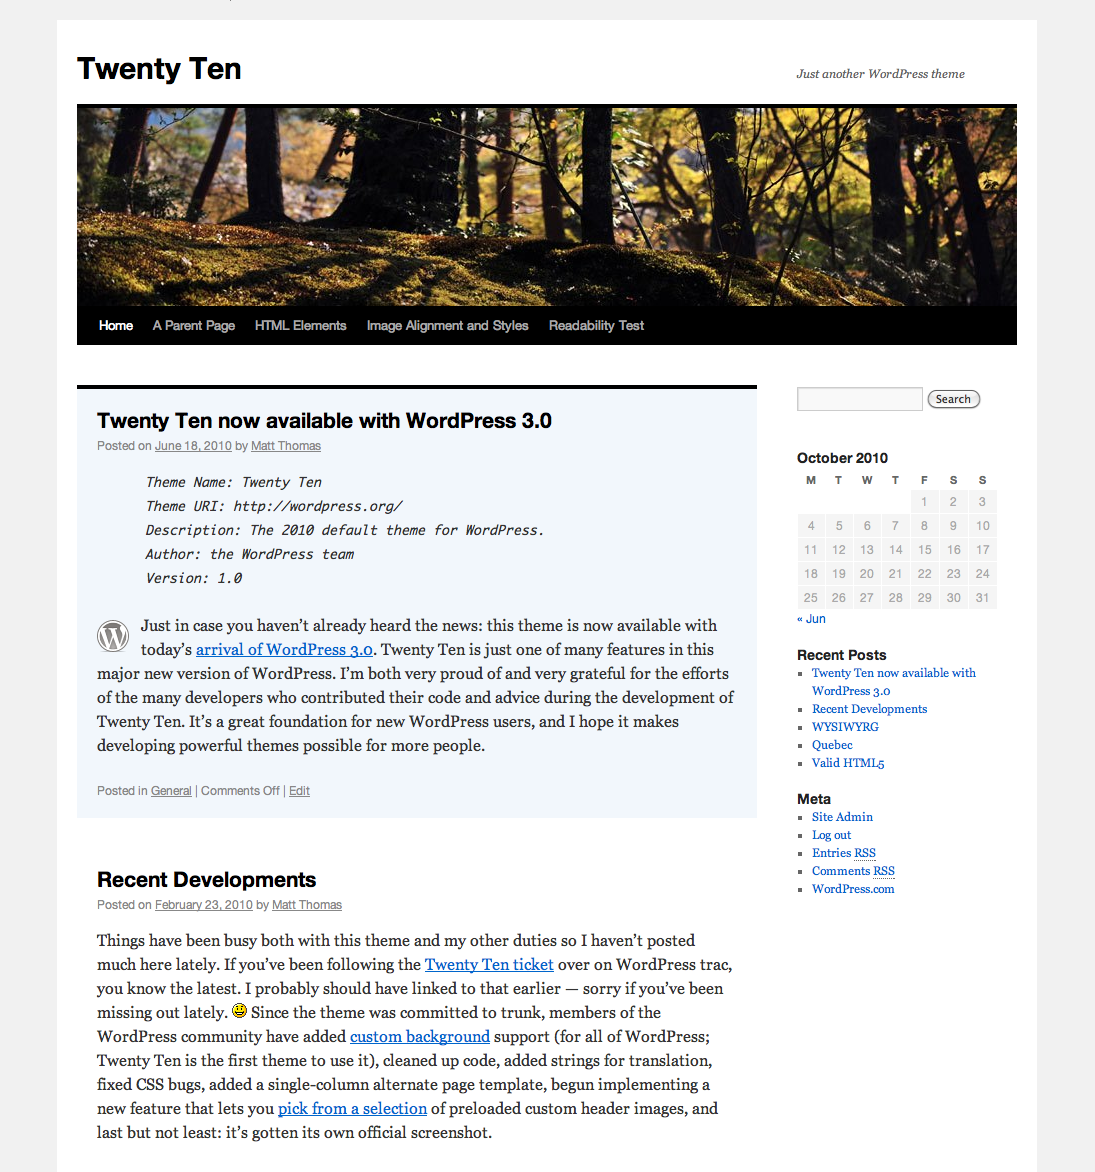
\includegraphics[width=\linewidth]{fig/wordpress}
\caption{Przykładowa strona wykonana w WordPress.}
\source{commons.wikimedia.org}
\end{figure}

\newpage

\section{Możliwości zastosowania praktycznego}

System TrainCMS został opracowany w taki sposób, aby sprostać wielu wymaganiom różnych użytkowników. Oferuje sporo możliwości, które przypadną do gustu każdemu i będą zarazem bardzo przydatne w codziennej pracy nad własna witryną Internetową. Reasumując, możliwości serwisu ogranicza jedynie wyobraźnia administratora.

\subsection{Strona wizytówka}

W celu stworzenia optymalnej i efektownej strony wizytówki należałoby uruchomić tryb statycznej strony głównej. W tymże celu utworzymy zakładkę, którą oznaczymy jako strona główna. Ilość pozostałych zakładek jest dowolna. Może się też zdarzyć potrzeba prowadzenia mini bloga lub prostych aktualności firmy, tutaj posłużymy się kategoriami i artykułami. Łącza do kategorii będą wyświetlone na górnym pasku nawigacji co ułatwi poruszanie się po stronie.  Po odpowiednim według operatora strony rozmieszczeniu informacji, możemy przejść do podglądu statystyk, które w tym przypadku mogą wyświetlić informację na przykład o tym, która sekcji informacji jest najbardziej popularna.

\subsection{Internetowe portfolio}

Każda osoba tworząca w Internecie portfolio swojej działalności zamierza przyciągnąć w ten sposób jak największą liczbę nowych klientów. Aby skutecznie rozwiązać ten problem, proponuję, każde dzieło zaprezentować w osobnym artykule. Natomiast informacje, które autor chciałby, aby były zawsze łatwo dostępne, umieścić w przygotowanych do tego zakładkach, do których to łącza będą wyświetlane na górnym pasku nawigacji. Można też przyjąć inne podejście do tego tematu, otóż ustawić stronę główną jako stronę statyczną, następnie utworzyć kategorię, do której łącze, podobnie jak do zakładek ukaże się na górnym pasku nawigacji, w której to umieścimy dzieła swojej działalności.

\subsection{Serwis informacyjny}

W tym rozwiązaniu znajdą zastosowanie wszystkie zaimplementowane w systemie funkcjonalności. Większość rozwiązań została wyprofilowana właśnie na tego typu zastosowania. Głównym szkieletem jest w tym przypadku możliwość tworzenia wielu kategorii, gdzie redaktor takiego serwisu, będzie mógł z pełną łatwością organizować wszystkie tematy poruszane na portalu i jednocześnie wszystkie artykuły z każdej kategorii będą wyświetlane na stronie głównej. Gorące tematy będzie można oznaczać jako wyróżnione i tym sposobem będą przez cały widoczne na szczycie karuzeli. Gość odwiedzający serwis z łatwością wejdzie w interakcję ze stroną poprzez system komentarzy, operator serwisu będzie mógł korzystać z przejrzystych statystyk i za ich pomocą analizować pracę portalu oraz planować dalszy jego rozwój. Z pomocą dla nowych gości przyjdą tagi, dzięki którym będzie można szybko wyszukać artykuły poruszające dany temat. Łatwiejsze stanie się planowanie różnego rodzaju imprez za pomocą wbudowanego kalendarza wydarzeń. Autor piszący artykuły dla serwisu nie będzie musiał zagłębiać się w panel zaplecza, na stronie głównej po zalogowaniu znajdzie skróty do najważniejszych funkcji takich jak nowy artykuł, lista własnych artykułów oraz lista komentarzy pod tymi artykułami. Jeżeli autor zechce,  ma możliwość wyłączenia komentarzy. Jeżeli nadejdzie taka potrzeba, możemy skorzystać z zaimplementowanego mechanizmu zakładek, które to, po utworzeniu wyświetlone będą na górnym pasku nawigacji.

\chapter{Projekt i analiza}

\newpage

\section{Diagram związków encji}

\begin{figure}[!tbh]
\centering
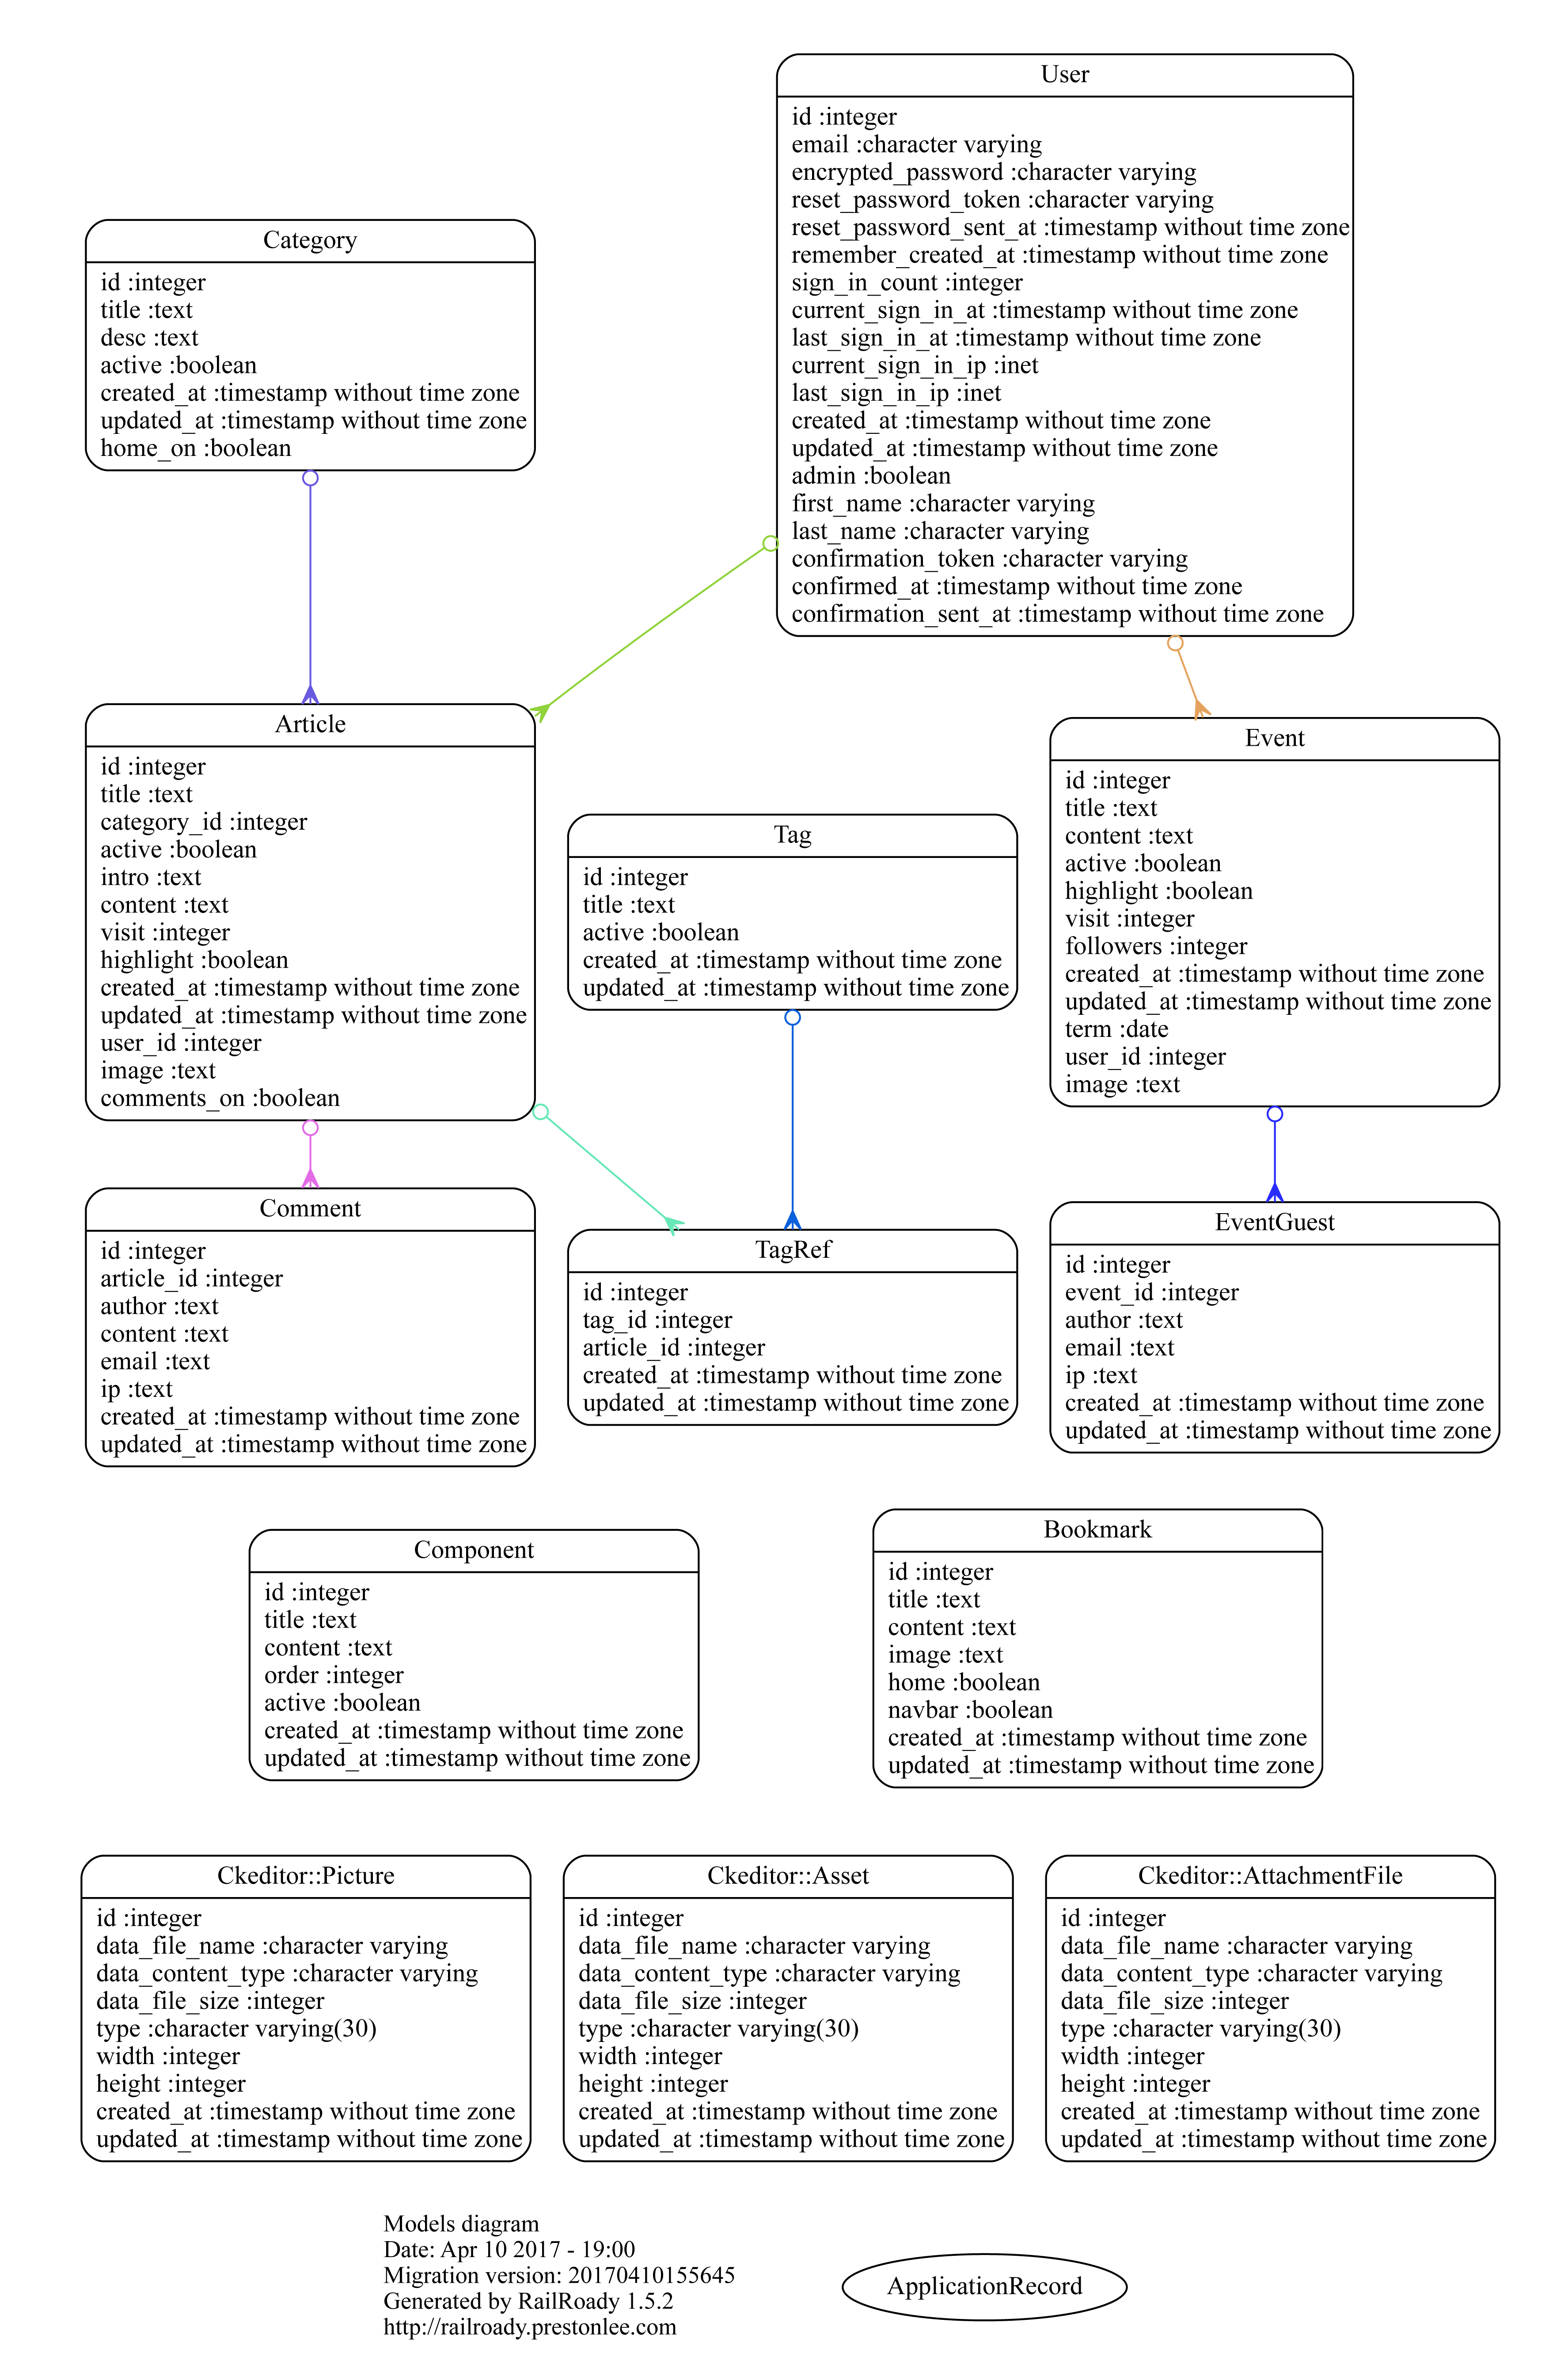
\includegraphics[width=.8\linewidth]{fig/erd2}
\caption{Diagram związków encji.}
\source{Opracowanie własne za pomocą i Gem RailRoady \cite{railroady}.}
\end{figure}

\section{Diagram kontrolera danych}
\begin{figure}[!tbh]
\centering
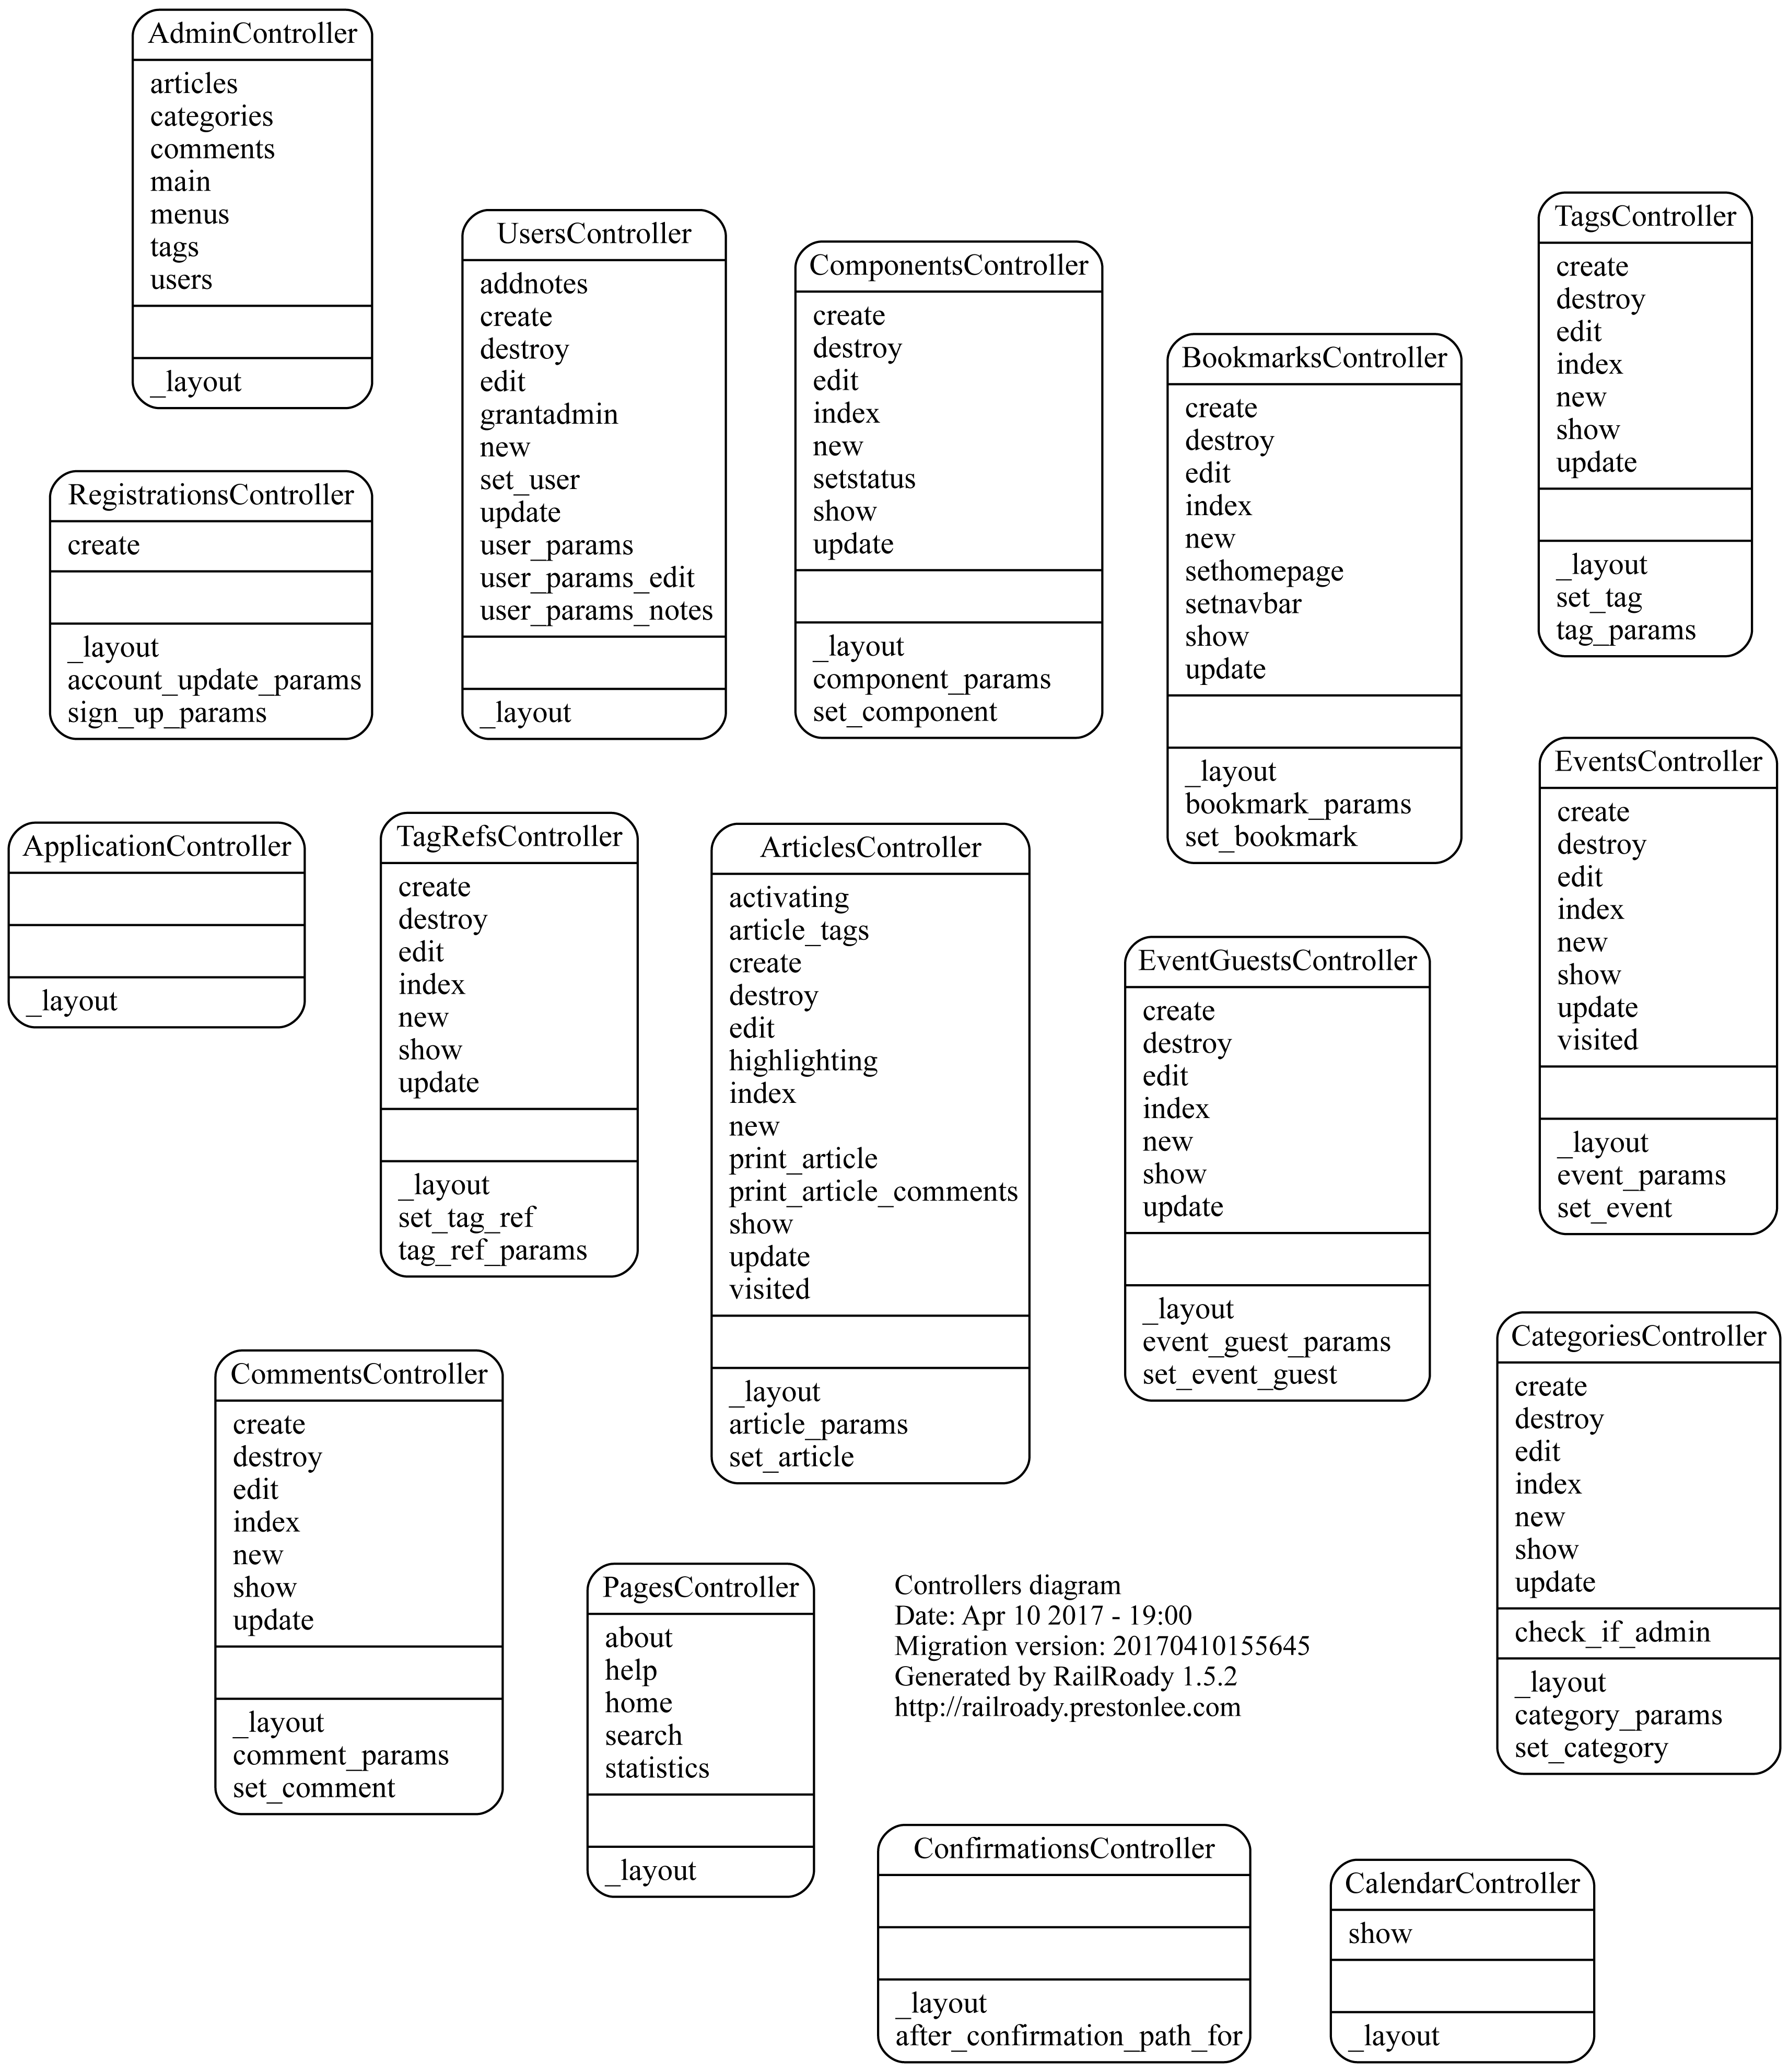
\includegraphics[width=.9\linewidth]{fig/controllers}
\caption{Diagram kontrolera danych.}
\source{Opracowanie własne  za pomocą i Gem RailRoady.}
\end{figure}

\newpage

\section{Diagram Przypadków Użycia}
\begin{figure}[!tbh]
\centering
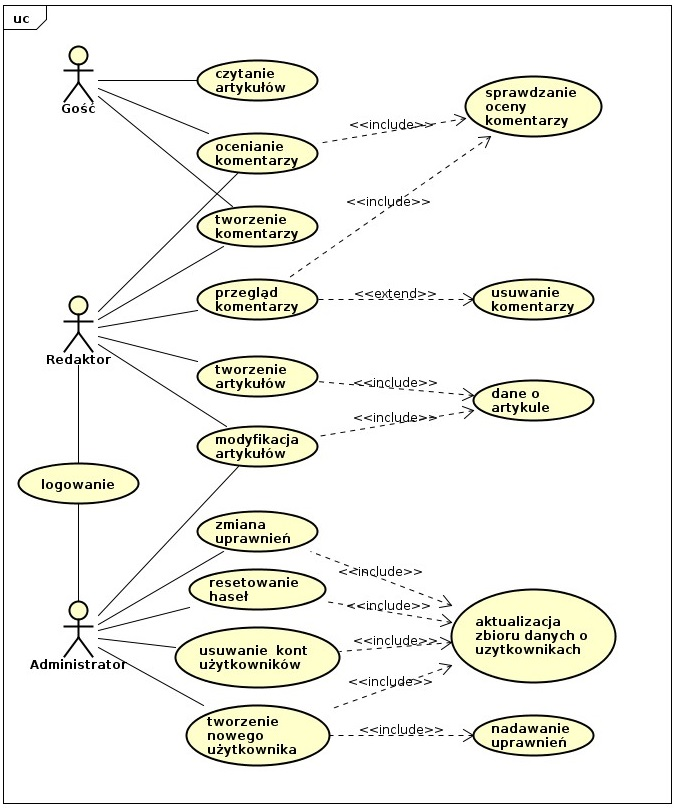
\includegraphics[width=.9\linewidth]{fig/uc}
\caption{Diagram Przypadków Użycia.}
\source{Opracowanie własne za pomocą programu Astah \cite{astah}.}
\end{figure}

\section{Projekt interfejsu użytkownika}

\subsection{Panel Administracyjny}
\begin{figure}[!tbh]
\centering
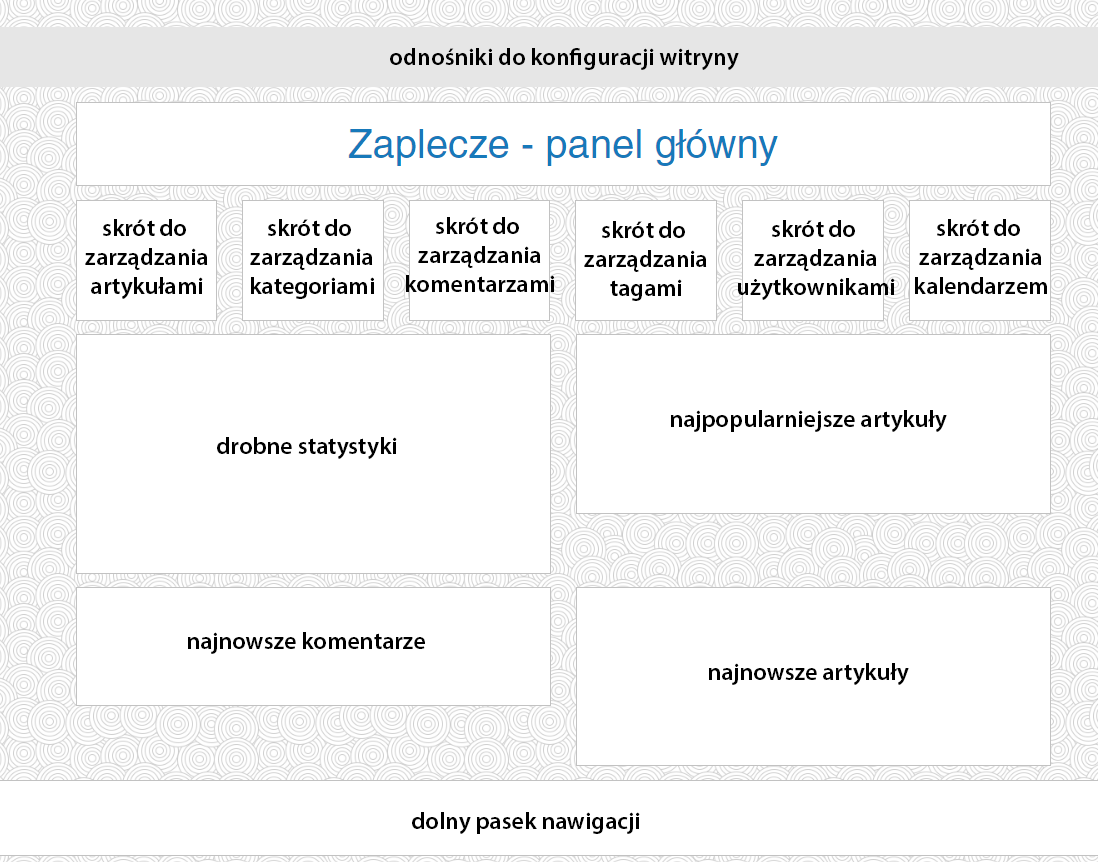
\includegraphics[width=.9\linewidth]{fig/gui_admin}
\caption{Projekt interfejsu użytkownika. Panel Administracyjny.}
\source{Opracowanie własne}
\end{figure}

\newpage

\subsection{Widok Redaktora}
\begin{figure}[!tbh]
\centering
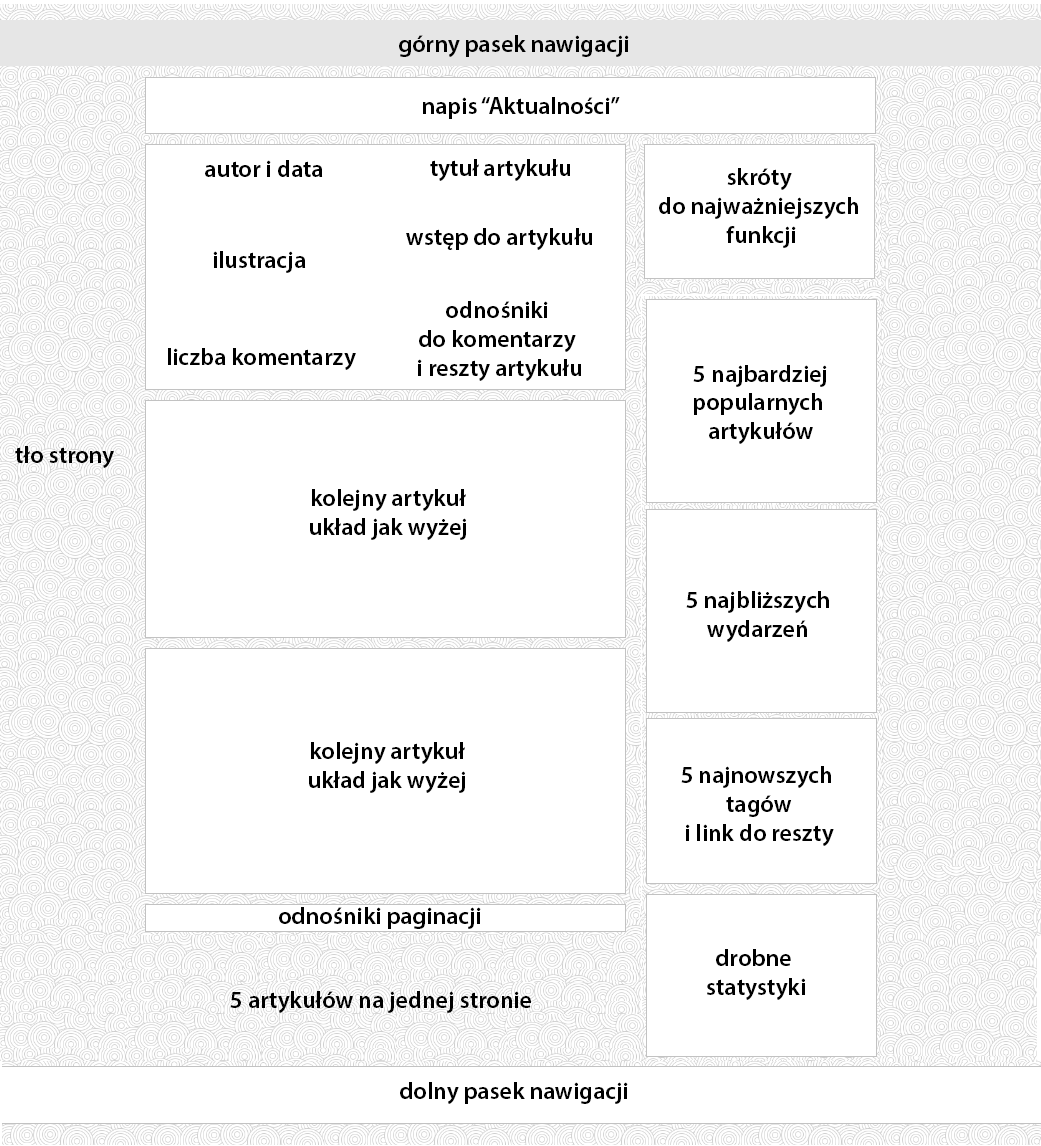
\includegraphics[width=.9\linewidth]{fig/gui_editor}
\caption{Projekt interfejsu użytkownika. Widok Redaktora.}
\source{Opracowanie własne}
\end{figure}

\newpage

\subsection{Widok Gościa}
\begin{figure}[!tbh]
\centering
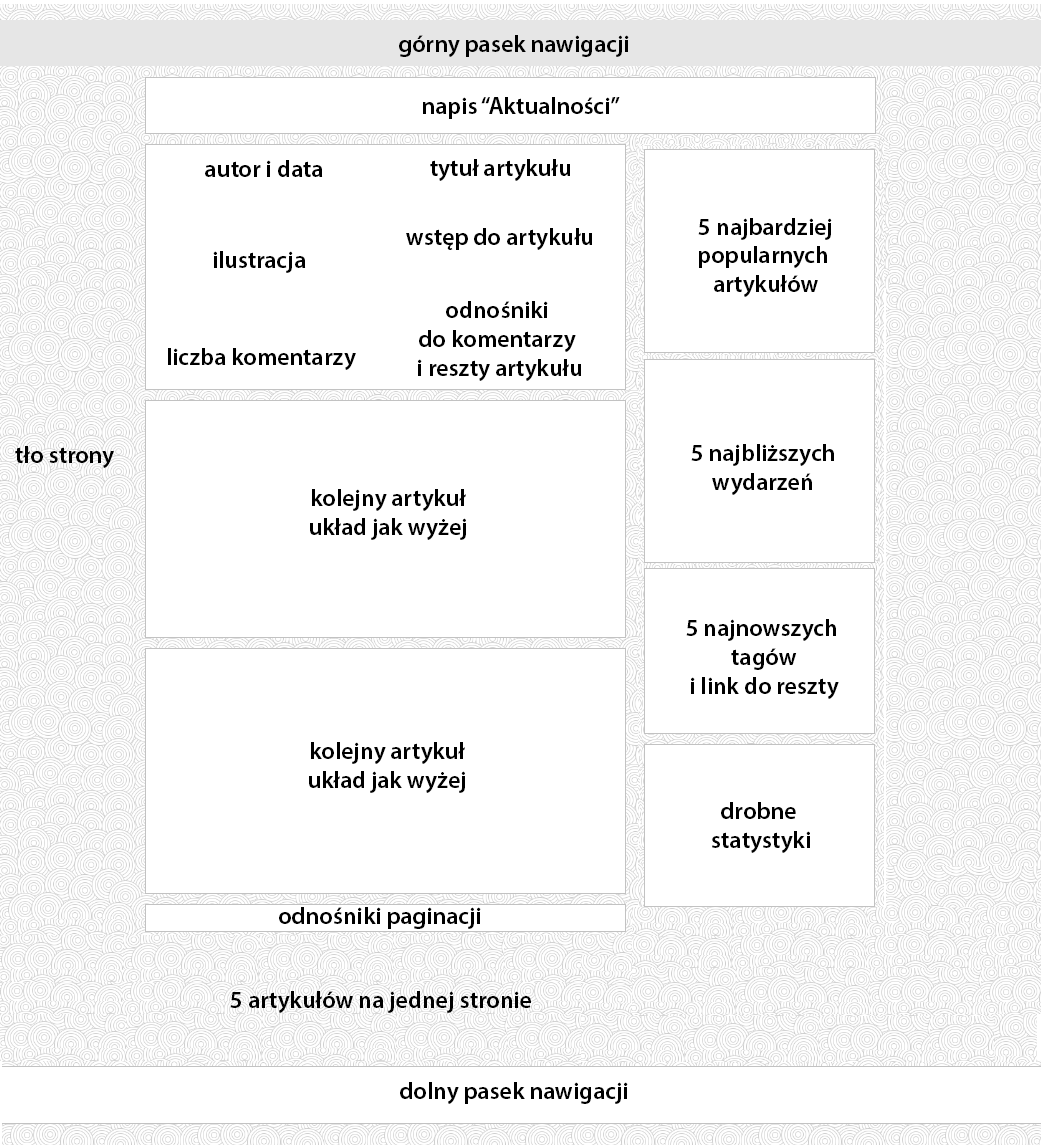
\includegraphics[width=.9\linewidth]{fig/gui_guest}
\caption{Projekt interfejsu użytkownika. Widok Gościa.}
\source{Opracowanie własne}
\end{figure}

\chapter{Implementacja}

\section{Architektura rozwiązania -- Ruby on Rails}
Głównym rusztowaniem całego systemu jest framework Ruby On Rails \cite{ror} \cite{enterprise} \cite{wikibook} \cite{guides}. Odpowiada on zarówno za frontend jak i backend. Do swojego działania używa bazy PostgreSQL. W dalszych podrozdziałach przybliżę jak wyglądała implementacja poszczególnych elementów systemu za pomocą Ruby On Rails. Framework dystrybuowany jest na licencji MIT License\footnote{MIT License -- Jest to jedna z najmniej rozbudowanych licencji oprogramowania i zarazem jest jedna z najbardziej liberalnych. Umożliwia nieograniczone prawo do użytkowania, kopiowania, modyfikowania i publikacji, również sprzedaży wersji pierwotnej bądź zmodyfikowanej oprogramowania. Jedynym wymaganiem jest umieszczenie informacji o autorze i licencji.}.

\subsection{Artykuły i Kategorie}
Podstawową jednostką na stronie jest artykuł, który zawsze zawiera się w jednej z uprzednio utworzonych kategorii. Artykuł posiada atrybuty takie jak tytuł, wstęp, treść główną, numer kategorii do której został przypisany, ilustrację, znacznik aktywności, znacznik wyróżnienia, znacznik komentarzy, liczbę wyświetleń oraz znaczniki czasowe – data, czas utworzenia i edycji. Chciałbym przybliżyć niektóre z atrybutów, pierwszym z nich będą znaczniki aktywności, wyróżnienia i komentarzy, które kolejno oznaczają informacje o tym, czy artykuł jest aktywny co przekłada się na to, że będzie wyświetlony na stronie głównej oraz spisie artykułów danej kategorii, kolejny atrybut determinuję to, czy artykuł zostanie wyświetlony na karuzeli ilustracji na szczycie strony głównej, ostatni ze znaczników pozwala dezaktywować moduł komentarzy w przypadku, gdyby zaszła konieczność, aby przy pewnym artykule nie miałoby być komentarzy. Liczba wyświetleń jest sumaryczną wartością wszystkich odsłon artykułu, obliczanie polega na pobraniu liczby wyświetleń z bazy danych, następnie zwiększeniu jej o jeden oraz aktualizacji wartości w bazie danych. Znaczniki czasowe są automatycznie dodawane przez Rails. Zarówno na stronie głównej, jak i na liście artykułów danej kategorii wyświetlany jest tytuł, wstęp do artykułu, ilustracja, autor, data utworzenia, liczba komentarzy. Po przejściu do artykułu zobaczymy pełną treść, w tym celu właśnie zostały zaimplementowane dwa oddzielne atrybuty. Zaimplementowana została również wyszukiwarka artykułów, gdzie słowem kluczowym wyszukiwania jest tytuł artykułu. Algorytm wyszukiwania ignoruje wielkość liter oraz pozwala wyszukiwać treści za pomocą fragmentów wyrazów. Artykuły mogą dodawać jedynie zalogowani użytkownicy. Po przejściu do artykułu możemy go wydrukować dzięki specjalnie do tego przygotowanej formatce optymalizującej miejsce na stronie kartki papieru.

Kategoria natomiast posiada atrybuty takie jak: tytuł, opis, znacznik aktywności, znacznik strony głównej oraz znaczniki czasowe – data, czas utworzenia i edycji. Wszystkie kategorie oznaczone jako aktywne wyświetlane są na górnym pasku nawigacji, po przejściu w odnośnik do danej kategorii zobaczymy opis kategorii oraz listę wszystkich artykułów przypisanych do tejże kategorii. Istnieje również taki atrybut jak znacznik strony głównej, który określa to czy artykuły przypisane do kategorii będą wyświetlane na stronie głównej. Do strony głównej może być przypisane kilka kategorii.

\subsection{Komentarze}
Do każdego artykułu możemy dodawać komentarze. Ta funkcjonalność udostępniona jest dla gości odwiedzających stronę, a co za tym idzie, aby dodać komentarz nie jest wymagane logowanie. W celu dodania komentarza musimy podać swój adres e-mail, który jednak nie będzie weryfikowany, jest to powszechnie stosowana praktyka. W bazie danych zapisywany jest także adres IP autora komentarza. Każdy komentarz można ocenić w skali plus/minus. Obok treści komentarza wyświetlana jest wartość oceny, która może być również ujemna. Jeden odwiedzający może ocenić jeden komentarz jeden raz, informacja o tym fakcie zapisywana jest w ciasteczkach.

\newpage

\subsection{Tagi}
W celu dodatkowej kategoryzacji oraz łatwiejszego znajdowania poszukiwanych przez odwiedzających treści, zaimplementowano tagi artykułów. Po utworzeniu artykułu, możemy przejść do formularza dodawania tagów, w którym za pomocą listy rozwijanej wybieramy dopasowane tagi, w tym samym miejscu, jeżeli nie znajdziemy poszukiwanych przez siebie tagów, możemy dodać swój tag i przypisać go do artykułu.

Implementacja tagów polegała na stworzeniu dwóch modeli. Pierwszy z nich odpowiedzialny jest za przechowywanie tagów jako samych w sobie, to znaczy w ich właściwej formie. Natomiast drugi model, odpowiada za relacje między tagiem a danym artykułem.

\subsection{Zakładki}
W celu uporządkowania statycznych informacji prezentowanych na stronie, zaimplementowano zakładki. Za pomocą atrybutów przypisanych do każdej zakładki możemy określać tytuł, treść, ilustrację, znacznik strony głównej, znacznik paska nawigacji oraz znaczniki czasowe – data, czas utworzenia i edycji. Znacznik strony głównej decyduje o tym, czy dana zakładka będzie pełniła rolę strony głównej. Natomiast znacznik paska nawigacji determinuje fakt wyświetlenia odnośnika do zakładki na górnym pasku nawigacji. Aby zakładka została wyświetlona na stronie głównej konieczne jest zaznaczenie tylko jednej zakładki w przypadku, gdy zostaną więcej niż dwie, wtedy strona główna przybierze formę dynamiczną.

\newpage

\subsection{Strona główna}
Strona główna może zostać skonfigurowana na dwa sposoby. Pierwszy sposób polega na wyświetlaniu listy artykułów oraz jej stronicowaniu, do którego służy Gem \texttt{will\_paginate}\cite{willpaginate}. Jak wcześniej wspomniałem na stronie głównej wyświetlone zostaną tylko artykuły aktywne z aktywnych kategorii. Każdy artykuł znajdzie się w osobnej ramce, w której znajdą się informacje o autorze, dacie publikacji, ilość komentarzy, tytuł oraz wstęp do artykułu, oraz także miniatura ilustracji artykułu i na dole odnośnik do formularza dodawania komentarza oraz odnośnik do właściwej treści artykułu. Na szczycie głównej witryny pojawi się również karuzela z wyróżnionymi artykułami a i wydarzeniami. Drugim sposobem aranżacji strony głównej jest jest statyczna wersja organizowana za pomocą wyżej opisanych zakładek. Strona przechodzi w ten tryb wtedy i tylko wtedy gdy tylko jedna zakładka ma znacznik strony głównej oznaczony jako prawda.

Na stronie głównej możemy umieszczać także komponenty, są to ramki z pewną treścią. Na stałe zostały osadzone cztery komponenty zawierające listę popularnych artykułów, listę najbliższych wydarzeń, listę najnowszych tagów oraz drobne statystyki. Komponenty za wzór innych modułów strony posiadają znacznik aktywności, który określa czy dany komponent będzie wyświetlony na stronie głównej.

Implementacja strony głównej polegała na stworzeniu osobnego pliku i rozmieszczeniu w nim w odpowiedni sposób wszystkich wymaganych składników strony. Za wyświetlanie komponentów odpowiada specjalna funkcja, która sprawdza ilość aktywnych komponentów, następnie na tej podstawie decyduje czy w ogóle wyświetlać którykolwiek komponent, nastąpi to po spełnieniu warunku mówiącego o ilości aktywnych komponentów więcej niż jeden. W przypadku kiedy nie wyświetlony zostaje żaden komponent, zmienia się szerokość listy artykułów lub szerokość wyświetlanej zakładki.

\newpage

\subsection{Kalendarz Wydarzeń}
Zaimplementowany został również kalendarz wydarzeń, który wyświetla dodane wydarzenia w formie klasycznego kalendarza ściennego, podzielonego na pojedyncze miesiące. Każde wydarzenie, na wzór artykułu, posiada atrybuty takie jak tytuł, treść, termin wydarzenia, ilustrację, znacznik aktywności, znacznik wyróżnienia, liczbę wyświetleń oraz znaczniki czasowe – data, czas utworzenia i edycji. Znaczniki aktywności i wyróżnienia są odpowiedzialne odpowiednio za wyświetlanie wydarzenia na kalendarzu oraz na liście pod kalendarzem.

Goście odwiedzający stronę mogę zapisywać się do wybranego przez siebie wydarzenia, polega to na podaniu swojego imienia oraz adresu e-mail, ponadto w tle do bazy danych trafia również adres IP osoby deklarującej dołączenie do wydarzenia. Wydarzenia mogą tworzyć jedynie zalogowani użytkownicy.

\begin{figure}[!tbh]
\centering
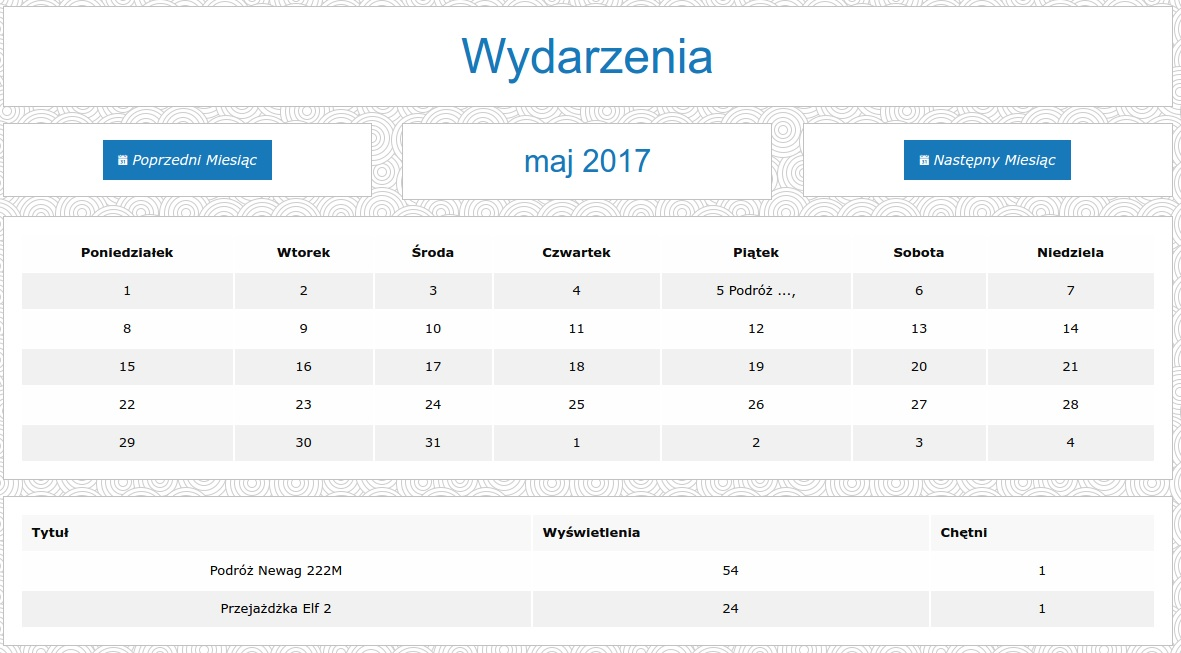
\includegraphics[width=\linewidth]{fig/events}
\caption{Widok kalendarza wydarzeń.}
\source{Opracowanie własne}
\end{figure}

\subsection{Nawigacja}
Nawigacja po stronie zrealizowana jest za pomocą dwóch pasków nawigacji, górnego i dolnego.

Na górnym pasku znajdziemy odnośniki do strony głównej, wszystkich kategorii oznaczonych jako te, które mają się znaleźć na pasku, zakładek, które podobnie jak kategorie muszą być oznaczone jako dostępne z poziomu paska nawigacji. Znajduje się tam również odnośnik do kalendarza wydarzeń oraz wyszukiwarki artykułów.

\begin{figure}[!tbh]
\centering

\includegraphics[width=\linewidth]{fig/navbar}
\caption{Przykładowy górny pasek nawigacji.}
\source{Opracowanie własne}
\end{figure}

Natomiast na dolnym pasku nawigacji zwanym stópką, znajduję się w widoku dla niezalogowanych użytkowników klauzula Copyright, odnośnik do planszy pod tytułem „o projekcie”, odnośnik do prostej pomocy oraz odnośnik do panelu logowania. Po zalogowaniu z uprawnieniami redaktora znajdziemy dodatkowo odnośnik do statystyk, natomiast po zalogowaniu z uprawnieniami administratora zyskamy odnośnik do zaplecza. Dla wszystkich zalogowanych użytkowników na prawym końcu dolnego paska nawigacji znajduje się odnośnik do panelu zmiany hasła oraz przycisk wylogowania.

\begin{figure}[!tbh]
\centering

\includegraphics[width=\linewidth]{fig/footbar}
\caption{Przykładowy dolny pasek nawigacji.}
\source{Opracowanie własne}
\end{figure}

\newpage

\subsection{Kanał RSS}
Kolejną zaimplementowaną w systemie funkcjonalnością jest agregator kanału RSS. Dzięki niemu fani witryny mogą dodać sobie link RSS do swojego czytnika i mieć zawsze dostęp do najnowszych informacja publikowanych na stronie.

Implementacja polegała na stworzeniu dwóch plików, jednego w standardzie Atom i jednego w standardzie RSS. Następnie wypełnieniu ich kodem wyświetlającym tytuł artykułu, nagłówek, autora oraz odnośnik do pełnej treści artykułu. Na obu plikach została przeprowadzona walidacja, która wykazała pozytywny wynik co oznacza, że są one w pełni zgodne z obowiązującymi wersjami obu standardów.

\begin{lstlisting}[language=ruby2, caption={Kod generatora spływu wiadomości w standardzie Atom}]
atom_feed do |feed|
  feed.title "TrainCMS - Artykuly"
  feed.updated @articles.maximum(:updated_at)
  @articles.order("created_at desc").each do |article|
    feed.entry article do |entry|
      entry.title article.title
      entry.content sanitize(article.intro, :tags => {})
      entry.author do |author|
        author.name
	User.where(id:article.user_id).pluck(:email).last
      end
    end
  end
end
\end{lstlisting}

\newpage

\section{ZURB Foundation}
ZURB Foundation \cite{foundation} to responsywny framework części wizualnej. Został stworzony w 2011 roku i dystrybuowany jest na licencji MIT License.

\subsection{Instalacja}
Aby dołączyć framework Foundation do projektu Ruby On Rails należy zainstalować Gem o nazwie \texttt{foundation-rails}. Następnie zainstalować go za pomocą polecenia
\begin{lstlisting}[language=html, caption={Kod instalujący Foundation w naszym projekcie}]
$ rails g foundation:install
\end{lstlisting}
oraz dodaniu odpowiednich zapisów w plikach kaskadowych arkuszy stylów i plikach skryptów JavaScript.

\subsection{Użycie}
Podczas budowy całego systemu zarządzania treścią strony internetowej korzystałem z bogatej biblioteki komponentów jaką oferuje framework Foundation. Każda zaimplementowana tabela otrzymała klasę
\begin{lstlisting}[language=html, caption={Przykładowa tabela}]
<table class="stack"></table>
\end{lstlisting}
która odpowiedzialna jest za wyświetlanie tabeli w mobilnym widoku jako stos kolumn, wiersze tabeli wyświetlane są na przemian kolor biały z kolorem grafitowym, tę funkcję również  zawdzięczamy Foundation. Wszystkie odnośniki \mbox{posiadają klasę}
\begin{lstlisting}[language=html, caption={Przykładowy przycisk}]
<%= link_to 'odnosnik', odnosnik_path,
	class:'button' %>
\end{lstlisting}
co pozwala na wyświetlanie każdego odnośnika w formie prostokątnego przycisku. Wszystkie odnośniki nie są przyciskami o tej samej wielkości, odnośniki zawarte na przykład w tabeli mają dodatkową klasę
\begin{lstlisting}[language=html, caption={Przykładowy mały przycisk}]
<%= link_to 'maly odnosnik', maly_odnosnik_path,
	class:'tiny button' %>
\end{lstlisting}
dzięki której przycisk staję bardzo mały i w elegancki sposób wkomponowuje się w wiersze tabeli. Również do nawigacji podczas stronicowania wykorzystano metodę renderowania w stylu Foundation. Ogólna konwencja graficzna opiera się na siatce, opisanej za pomocą znaczników \texttt{div}. Każda sekcja wszystkich stron poszczególnych modułów całego systemu zapisana jest w znaczniku \texttt{div}, który otrzymuje za każdym razem klasę
\begin{lstlisting}[language=html, caption={Przykładowy div}]
<div class="callout"></div>
\end{lstlisting}
Dzięki, której treść wyświetlana jest na białym eleganckim prostokącie z ostrymi rogami. Strona główna została podzielona za pomocą siatki znaczników \texttt{div} na kilka sekcji. Formularze wprowadzania danych wykorzystują klasę \texttt{div}
\begin{lstlisting}[language=html, caption={Przykładowe pole tekstowe}]
<div class="input-group">
	<span class="input-group-label">Tytul</span>
         <%= f.text_field :title, type:"text",
		class:"input-group-field" %>
</div>
\end{lstlisting}
która pozwala na wyświetlanie etykiety i samego pola w jednej linii, oszczędzając tym samym miejsce, prezentując stronę w jeszcze bardziej czytelny sposób.

\subsection{Ikony}
Bardzo ciekawą funkcjonalnością Foundation jest możliwość dodawania ikon w kodzie strony. W tym celu należy zainstalować Gem o nazwie Foundation Icon Fonts on SASS for Rails \cite{icons}, potrzebne do tego będzie dodanie wpisu do pliku Gemfile oraz dodania linii kodu do pliku \texttt{application.css.scss} znajdującego się w katalogu \texttt{app/assets/stylesheets/}:
\begin{lstlisting}[language=ruby2, caption={Kod dołączający zbiór ikon Foundation Icons do aplikacji}]
@import 'foundation-icons';
\end{lstlisting}
Na koniec w celu wyświetlenia ikony na stronie, należy dodać kod, którego wynikiem będzie ikona kalendarza wielkości 24 punktów:
\begin{lstlisting}[language=html, caption={Przykładowa ikona ze zbioru ikon Foundation Icons}]
<font size="24"><i class="fi-calendar"></i></font>.
\end{lstlisting}

\begin{figure}[!tbh]
\centering

\includegraphics{fig/icon}
\caption{Ikona kalendarza ze zbioru ZURB Foundation Icons.}
\source{Opracowanie własne}
\end{figure}

\newpage

\section{CarrierWave, CKEditor, Cloudinary}
\subsection{CarrierWave i Cloudinary}
CarrierWave \cite{carrierwave} jest to Gem usprawniający obsługę plików o różnych rozszerzeniach dla aplikacji w Ruby, natomiast Cloudinary jest to usługa oferująca przechowywanie plików na bezpłatnym serwerze hostingowym, dodatkowo o tej samej nazwie istnieje Gem \cite{cloudinary}, który obsługuje całą tę funkcjonalność z poziomu aplikacji Ruby. Oba rozwiązania są ze ściśle sobą powiązane, ale mogą też działać samodzielnie. Oba dodatki udostępnione są na licencji MIT License.

Gem należy dodać do pliku Gemfile. Następnie utworzyć plik uploader za pomocą polecenia:
\begin{lstlisting}[language=bashes, caption={Polecenie generujące plik uploader}]
$ rails generate uploader Avatar
\end{lstlisting}
które wygeneruje plik, w którym to możemy przeprowadzić konfigurację. Dodatkowo do swojego pełnego działania potrzebuje pakiet RMagick, który możemy zainstalować za pomocą polecenia systemowego:
\begin{lstlisting}[language=bashes, caption={Polecenie instalujące oprogramowanie RMagick}]
$ sudo apt-get install imagemagick libmagickwand-dev
\end{lstlisting}
Przed przejściem do dalszych kroków, potrzebne będzie konto w serwisie Clodinary, z tego też serwisu po zalogowaniu pobieramy plik konfiguracyjny przygotowany dla aplikacji napisanych w Ruby, zapisujemy go w katalogu \texttt{/config}. Do każdego z pliku uploadera, należy dodać dwie linie
\begin{lstlisting}[language=ruby2, caption={Fragment zawartości pliku uploader}]
include CarrierWave::Rmagick
include Cloudinary::CarrierWave.
\end{lstlisting}

\newpage

W celu zachowania porządku na serwerze usługi Cloudinary w każdym pliku uploader możemy dodać linię, która oznacza tagiem każdy załadowany przez nas plik:
\begin{lstlisting}[language=ruby2, caption={Przykładowy tag dla pliku}]
process :tags => ['random_tag']
\end{lstlisting}
Aby wyświetlić załadowany plik, na przykład obraz należy dodać linię o treści:
\begin{lstlisting}[language=ruby2, caption={Kod wyświetlający obraz}]
<%= image_tag @article.image.url %>
\end{lstlisting}

\subsection{CKEditor}
CKEditor \cite{ckeditor} jest edytorem WYSIWYG\footnote{\textit{ang. what you see is what you get} skrót oznaczający ,,to co widzisz, to otrzymasz", stosowany w technikach komputerowych do określenia rozwiązań pozwalających uzyskać już podczas produkcji tekstu wynik wielce zbliżony lub niemalże identyczny do finalnego efektu.}, który umożliwia łatwą i przejrzystą edycję tekstu w oknie przeglądarki, możliwościami zbliżonymi do edytora tekstu klasy Microsoft Word. Gem udostępniony jest na licencji MIT License.

W celu instalacji należy dodać Gem do pliku Gemfile. W drugim kroku należy dodać do pliku \texttt{config/initializers/ckeditor.rb} linie:
\begin{lstlisting}[language=ruby2, caption={Fragment zawartości pliku ckeditor.rb}]
Ckeditor.setup do |config|
  config.cdn_url =
	"//cdn.ckeditor.com/4.6.1/basic/ckeditor.js"
end
\end{lstlisting}

\newpage

Następnie w pliku \texttt{/app/views/layouts/application.html.html} linię o następującej treści:
\begin{lstlisting}[language=ruby2, caption={Fragment zawartości pliku application.html.rb}]
<%= javascript_include_tag "chartkick" %>
\end{lstlisting}
W miejscu, w którym chcemy użyć ten komponent dodajemy linię o treści:
\begin{lstlisting}[language=ruby2, caption={Kod uruchamiający edytor}]
<%= f.cktext_area :content, placeholder:"Content" %>
\end{lstlisting}
Rozwiązanie to ściśle współpracuje z przedstawionym wyżej rozwiązaniem publikacji załączników, na przykładzie artykułów, możemy nie tylko dodać główną ilustrację publikacji, ale także za pomocą CKEditor dodać kilka innych załączników, nie tylko obrazków, które także znajdą się na serwerze usługi Cloudinary.

\begin{figure}[!tbh]
\centering
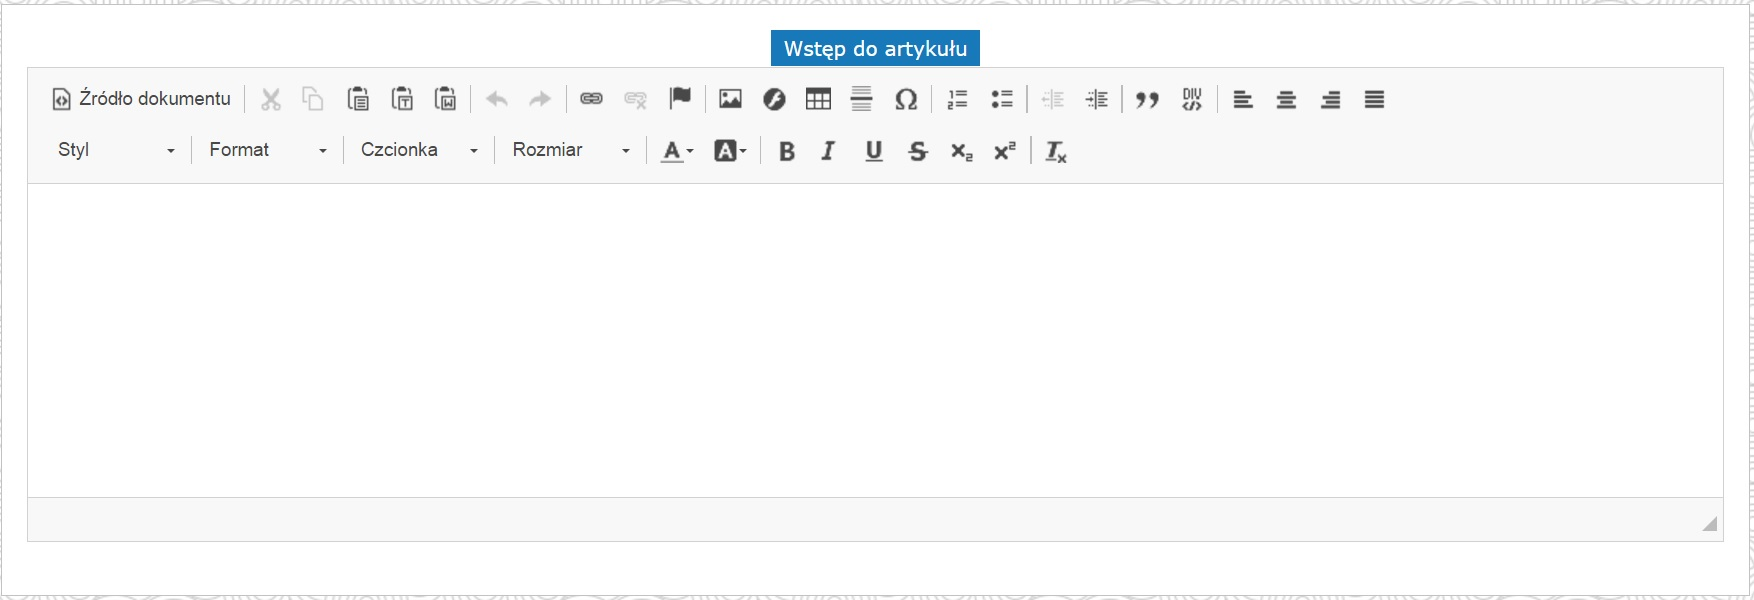
\includegraphics[width=\linewidth]{fig/ckeditor}
\caption{Edytor CKEditor.}
\source{Opracowanie własne}
\end{figure}

\newpage

\section{Prawn}
Prawn \cite{prawn} jest to Gem generujący pliki w formacie PDF. Udostępniano został na licencji GPL.

Aby zainstalować Gem w naszym projekcie, należy go dodać do pliku Gemfile. W celu utworzenia plików PDF należy utworzyć klasę w kontrolerze, która będzie dziedziczyła z klas komponentu:
\begin{lstlisting}[language=ruby2, caption={Deklaracja klasy generującej plik PDF}]
class ArticleOnePdf < Prawn::Document
\end{lstlisting}
Wykorzystanie Prawn umożliwia bardzo precyzyjne, pod względem rozmieszczania poszczególnych elementów, projektowanie dokumentów. Do generowanych dokumentów możemy dodawać obrazy, tabelę  i wiele innych elementów. Podczas generowania precyzujemy rozmiar oraz orientację strony.
\begin{lstlisting}[language=ruby2, caption={Kod generujący dokument zawierający ilustrację i wstęp do artykułu}]
class ArticleOnePdf < Prawn::Document
  def initialize(article)
    super()
    @article = article

    move_down 10
    photo = "#{Rails.root}/public#{@article.image.url}"
    image photo, :width => 400

    move_down 10
    font("SourceSansPro-Bold.ttf", size: 14) do
      text "#{remove_html(@article.intro)}"
  end
end
\end{lstlisting}

\newpage

\section{Chartkick}
Chartkick \cite{chartkick} to Gem, który z pewnością wzbogaci wizualnie każdy projekt, w którym się znajdzie. Jego głównym zadaniem jest generowanie wykresów. Pierwszy raz został opublikowany w 2013 i teraz udostępniany jest na licencji \mbox{MIT License. }

Aby zainstalować Gem należy dodać go do pliku Gemfile, następnie w pliku \texttt{application.js} dodać linię
\begin{lstlisting}[language=ruby2, caption={Fragment zawartości pliku application.js}]
//= require chartkick
\end{lstlisting}
natomiast w pliku \texttt{layouts/application.html} dodać linię:
\begin{lstlisting}[language=html, caption={Fragment zawartości pliku application.html.rb}]
<%= javascript_include_tag "//www.google.com/jsapi",
"chartkick" %>
\end{lstlisting}

Bardzo ciekawym wykresem jest wykres o nazwie \texttt{pie\_chart}. Można go umieścić w następujący sposób:
\begin{lstlisting}[language=html, caption={Kod generujący wykres kołowy}]
<%= pie_chart Article.group(:title).sum(:visit) %>
\end{lstlisting}

\newpage

Generuje on bardzo przejrzysty obrazek z wykresem kołowym:
\begin{figure}[!tbh]
\centering
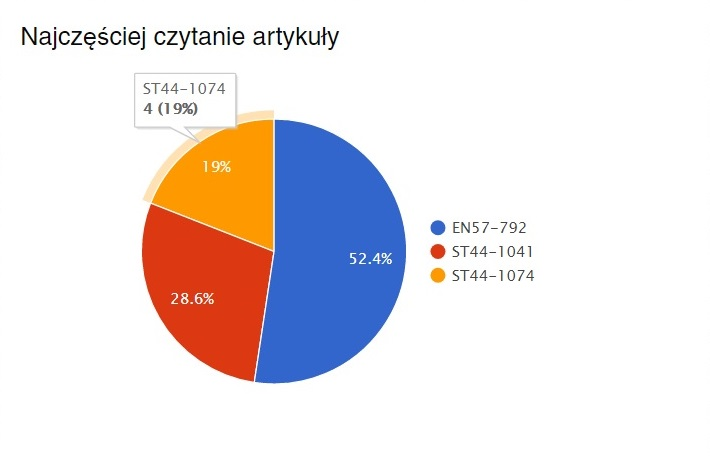
\includegraphics[width=.8\linewidth]{fig/chartkick}
\caption{Wykres kołowy.}
\source{Opracowanie własne}
\end{figure}

\section{reCAPTCHA}

W celu rozwiązania problemu zabezpieczenia systemów wdrożonych w ogólnodostępnej sieci Internet przed różnymi formami złośliwego oprogramowania, a szczególnie robotów spamujących za pomocą formularzy zawartych na stronach internetowych, wdrożyłem rozwiązanie o nazwie reCAPTCHA produkcji Google. W tym celu dodałem Gem o tej samej nazwie \cite{recaptcha} dystrybuowany na licencji MIT License.

\newpage

Instalacja polega na dodaniu wpisu do pliku Gemfile, zarejestrowaniu strony na serwerach Google w celu pobrania kodu strony i kodu sekretnego, które to należy dodać do pliku \texttt{/config/initializers/recaptcha.rb}. Następnie dodaniu do formularza linii kodu:
\begin{lstlisting}[language=ruby2, caption={Kod wyświetlający formularz reCAPTCHA}]
<%= recaptcha_tags %>
\end{lstlisting}
Na koniec należy dodać do pliku kontrolera poniższy fragment kodu:
\begin{lstlisting}[language=ruby2, caption={Kod kontrolera weryfikujący reCAPTCHA}]
if !verify_recaptcha
     flash.delete :recaptcha_error
     build_resource(comment_params)
     resource.valid?
     resource.errors.add(:base, "Proszę zaznaczyć Captcha.")
     clean_up_passwords(resource)
     respond_with_navigational(resource) { render :new }
else
      flash.delete :recaptcha_error
      super
end
\end{lstlisting}

\begin{figure}[!tbh]
\centering
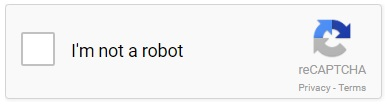
\includegraphics[width=.6\linewidth]{fig/captcha}
\caption{Formularz weryfikacyjny reCAPTCHA.}
\source{Opracowanie własne}
\end{figure}

\newpage

\section{Devise}
W celu organizacji uprawnień i dostępu do elementów strony przez upoważnione osoby zaimplementowano obsługę użytkowników. Całość polega na tym, aby dodać do naszego projektu Gem Devise\cite{devise}, który jest udostępniony na licencji MIT License. Natomiast jego instalacja polega na dodaniu go do pliku Gemfile, następnie użyciu generatora wbudowanego w Gem za pomocą polecenia powłoki:
\begin{lstlisting}[language=bashes, caption={Polecenie instalujące Gem Devise w naszym projekcie}]
$ rails generate devise:install
\end{lstlisting}
Kolejnym krokiem jest wygenerowanie modelu za pomocą następnego polecenia powłoki:
\begin{lstlisting}[language=bashes, caption={Polecenie generujące model użytkowników w naszym projekcie}]
$ rails generate devise users
\end{lstlisting}
Na koniec instalacji należy wykonać migracje bazy danych.

W przypadku TrainCMS, na tym nie zakończyła się implementacja obsługi użytkowników. Wprowadzono uprawnienia administratora, polegało to na stworzeniu metody w kontrolerze użytkowników, która to modyfikuje pole w bazie danych. Następnie w miejscach do których ma mieć dostęp tylko administrator, dane pole jest sprawdzane pod kątem występowania twierdzenia, wówczas użytkownik otrzymuje dostęp. Stworzono dodatkową podstronę w panelu administratora w celu zarządzania użytkownikami, na tejże stronie możemy usunąć danego użytkownika, nadać mu uprawnienia administratora, przejść do edycji jego danych oraz przejść do formularza dodawania użytkowników. W tym miejscu należy wspomnieć o założeniu, które twierdzi, że tylko administrator może dodawać użytkowników, nikt nie może się sam zarejestrować.

\begin{figure}[!tbh]
\centering
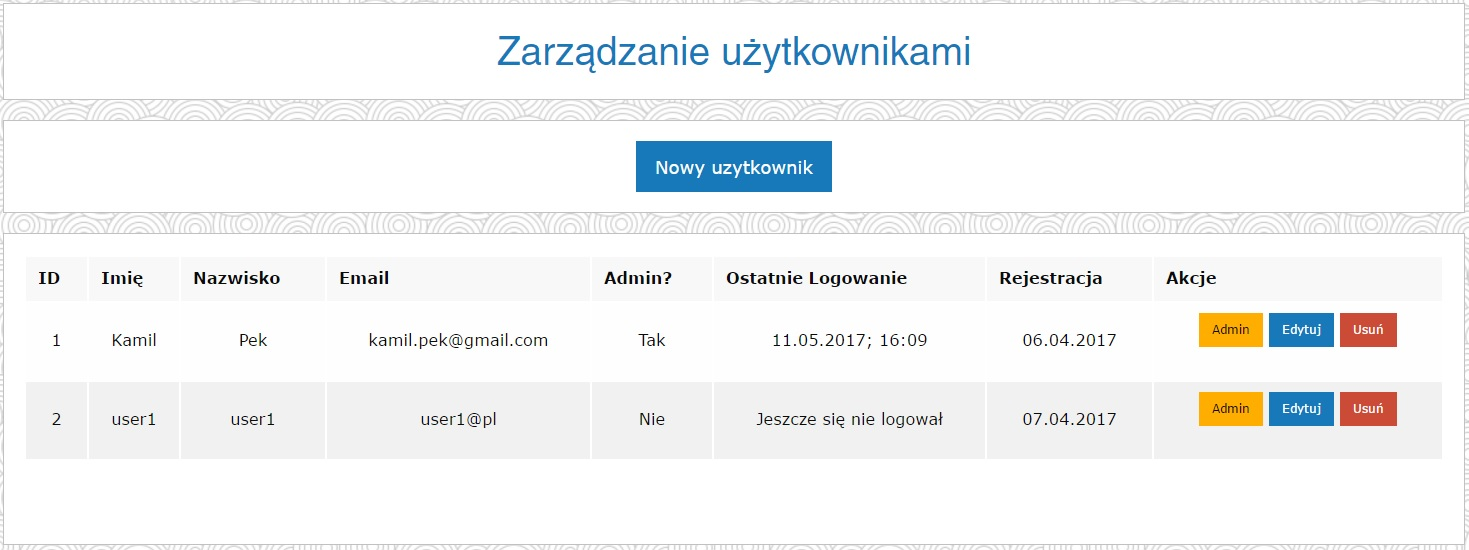
\includegraphics[width=\linewidth]{fig/uzytkownicy}
\caption{Widok panelu zarządzania użytkownikami.}
\source{Opracowanie własne}
\end{figure}

\newpage

\section{rQRcode i Prawn/QRCode}
Aby ułatwić promocję strony zaimplementowana została funkcjonalność generowania kodów QR, w tym celu z pomocą przychodzi Gem rQRcode\cite{rqrcode} i Gem Prawn/QRCode\cite{prawnqr}. Pierwszy Gem jest głównym silnikiem kodów QR w naszym projekcie, natomiast drugi Gem odpowiada za poprawne osadzanie kodu w dokumencie PDF. Instalacja polega na dodaniu obu dodatków do pliku Gemfile. Następnie należy dodać do pliku  \texttt{app/helpers/application.rb} linię:
\begin{lstlisting}[language=ruby2, caption={Kod dołączający rQRcode do projektu}]
require 'rqrcode'
\end{lstlisting}
Generowanie kodu QR polega na wywołaniu w kodzie strony polecenia:
\begin{lstlisting}[language=ruby2, caption={Kod generujący kod QR}]
qrcode = RQRCode::QRCode.new( ‘random text’ )
\end{lstlisting}

W systemie TrainCMS kody QR odpowiadają za prezentację odnośnika do strony danego artykułu. Umieszczone są one na wydruku artykłu oraz w pliku PDF z artykułem.

W celu wyświetlenia wygenerowanego kodu QR należy go skonwertować do formatu PNG za pomocą metody \texttt{as\_png}:
\begin{lstlisting}[language=ruby2, caption={Kod konwertujący kod QR}]
qrimage = qrcode.as_png
\end{lstlisting}
Następnie wyświetleniu go na stronie za pomocą polecenia:
\begin{lstlisting}[language=html, caption={Kod wyświetlający kod QR na stronie HTML}]
<img src="<%=@qrimage.to_data_url %>"/>
\end{lstlisting}
Aby umieścić kod QR w dokumencie PDF nalży dodać linię:
\begin{lstlisting}[language=ruby2, caption={Kod wyświetlający kod QR w dokumencie PDF}]
render_qr_code(qrcode)
\end{lstlisting}

Wygenerowany kod QR.
\begin{figure}[!tbh]
\centering

\includegraphics[width=.6\linewidth]{fig/kodqr}
\caption{Wygenerowany kod QR.}
\source{Opracowanie własne}
\end{figure}

\section{Geocoder}
Kolejnym ciekawym dodatkiem do projektu jest Gem Geocoder\cite{geocoder}, udostępniany na licencji MIT license. Pozwala on na tak zwane geokodowanie, czyli ustalanie za pomocą na przykład adresu  urzędowego współrzędnych geograficznych, tyczy się to również adresów IP z którymi radzi sobie nieco gorzej aniżeli z urzędowymi adresami.

Instalacja polega na dodaniu wpisów do pliku Gemfile. Każdy model, który ma zostać poddany geokodowaniu musi posiadać kolumny przeznaczone na przechowywanie długości i szerokości geograficznej. Następnie w pliku danego modelu dodajemy dwie linie kodu:
\begin{lstlisting}[language=ruby2, caption={Kod odpowiadający za geokodowanie}]
geocoded_by :adress
after_validation :geocode
\end{lstlisting}
Aby wyświetlić zlokalizowane koordynaty korzystamy z poleceń:
\begin{lstlisting}[language=ruby2, caption={Kod wyświetlający koordynaty}]
<%= @event.latitude %>, <%= @event.longitude %>
\end{lstlisting}
Funkcjonalność geokodowania została wdrożona przy kalendarzu wydarzeń, podczas tworzenia wydarzenia podajemy jego adres, a Gem ustala jego koordynaty, następnie w podglądzie danego wydarzenia uzyskujemy odnośnik do mapy z zaznaczoną pozycją geograficzną.

\begin{figure}[!tbh]
\centering

\includegraphics[width=\linewidth]{fig/geocoder-events}
\caption{Adres, koordynaty i odnośnik do mapy przy wydarzeniu}
\source{Opracowanie własne}
\end{figure}

Innym miejscem wdrożenia geokodowania jest moduł komentarzy. Gem na podstawie adresu IP ustala przybliżone współrzędne geograficzne, jednak należy pamiętać, że jest to tylko informacja o sugerowanym położeniu w rzeczywistości zgadza się tylko kraj co i tak nie jest wiążące, szczególnie kiedy użytkownik korzysta z usług VPN.

\begin{figure}[!tbh]
\centering
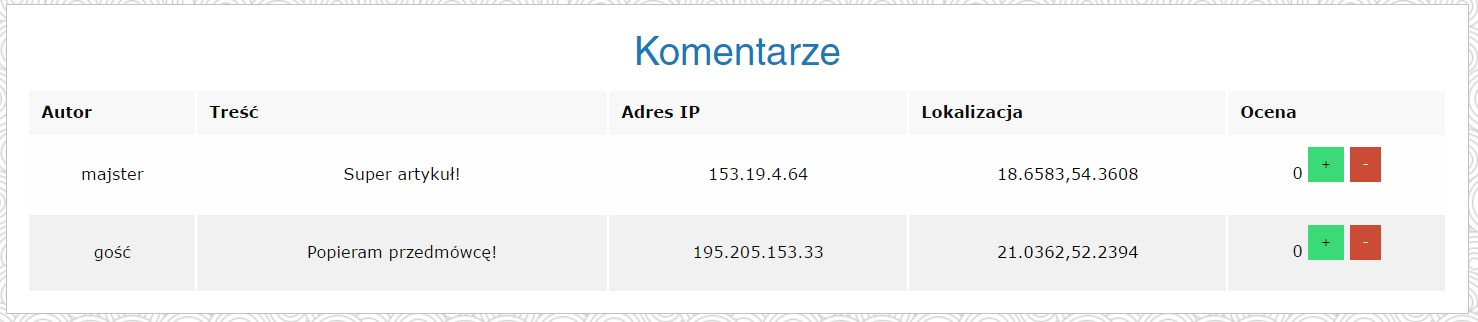
\includegraphics[width=\linewidth]{fig/geocoder-comments}
\caption{Koordynaty jako odnośnik do mapy przy komentarzach}
\source{Opracowanie własne}
\end{figure}

Opisany Gem posiada jeszcze sporo innych ciekawych funkcjonalności. Jedna z nich jest na przykład geokodowanie odwrotne. Polega to na podaniu pozycji geograficznej i na jej podstawie zaprezentowaniu adresu. Umożliwia on nam także obliczanie odległości w linii prostej pomiędzy punktami na pozycjami geograficznymi, wyznacza kierunek geograficzny za pomocą stopni. Gem przyjmuje również zapytania kierowane za pomocą konsoli. Odpowiedzi otrzymane na zapytania o  adres możemy w łatwy sposób podzielić na drobne parametry w przypadku adresów położonych w Stanach Zjednoczonych takie jak na przykład ulica, miasto, stan i kilka innych parametrów.

\newpage

\section{cookies\_eu}
Zgodnie z nowelizacją Prawa Telekomunikacyjnego uchwaloną dnia 16 listopada 2012 każdy operator strony internetowej zobowiązany jest do umieszczenia stosownej informacji o przechowywaniu i operowaniu na plikach cookies, potocznie zwanymi ciasteczkami. Z pomocą w wykonaniu tych obostrzeń przychodzi Gem cookies\_eu\cite{cookies}, udostępniany na licencji MIT license.

Instalacja polega na dodaniu wpisu do pliku Gemfile, następnie dodaniu do pliku app/assets/javascripts/application.js jednej linii kodu o następującej treści:
\begin{lstlisting}[language=ruby2, caption={Kod odpowiadający za dodanie bibliotek javascript}]
//= require cookies_eu
\end{lstlisting}
Natomiast do pliku app/asstes/stylesheets/aplication.css linii kodu o treści:
\begin{lstlisting}[language=ruby2, caption={Kod odpowiadający za dodanie bibliotek kaskadowych arkuszy stylów}]
*= require cookies_eu
\end{lstlisting}
Na koniec dodajemy linię, która będzie odpowiadać za renderowania paska ze stosowną informacją na dole strony:
\begin{lstlisting}[language=ruby2, caption={Kod renderujący pasek z informacją o ciasteczkach}]
<%= render 'cookies_eu/consent_banner' %>
\end{lstlisting}

Wynik końcowy prezentuje się w następujący sposób:
\begin{figure}[!tbh]
\centering

\includegraphics[width=\linewidth]{fig/cookies}
\caption{Belka informująca o plikach cookies.}
\source{Opracowanie własne}
\end{figure}


\begin{thebibliography}{9}
\bibitem{ror}
John Elder.
\textit{Learn Ruby On Rails For Web Development: Learn Rails The Fast And Easy Way!}.
Codemy.com; 1 edition (January 19, 2015).

\bibitem{enterprise}
Dan Chak.
\textit{Enterprise Rails}.
O'Reilly Media; 1 edition (November 3, 2008).

\bibitem{wikibook}
Użytkownicy Wikibooks.
\textit{Ruby}.
Wikibooks; 1 edition (February 17, 2008).

\bibitem{railroady}
Oficjalna dokumentacja - Gem RailRoady.
\\\texttt{\url{http://railroady.prestonlee.com/}} (dostęp 22.05.2017)

\bibitem{astah}
Oficjalna dokumentacja Aplikacji Astah.
\\\texttt{\url{http://astah.net/tutorials}} (dostęp 22.05.2017)

\bibitem{guides}
Oficjalna dokumentacja frameworku Ruby on Rails.
\\\texttt{\url{http://guides.rubyonrails.org/}} (dostęp 22.05.2017)

\bibitem{api}
Oficjalna dokumentacja API Ruby on Rails.
\\\texttt{\url{http://api.rubyonrails.org/}} (dostęp 22.05.2017)

\bibitem{willpaginate}
Oficjalna dokumentacja - Gem will\_pagintate.
\\\texttt{\url{http://www.rubydoc.info/gems/will_paginate/}} (dostęp 22.05.2017)

\bibitem{foundation}
Oficjalna dokumentacja frameworku Foundation for Sites.
\\\texttt{\url{http://foundation.zurb.com/sites/docs/}} (dostęp 22.05.2017)

\bibitem{icons}
Oficjalna dokumentacja - Gem Foundation Icon.
\\\texttt{\url{http://www.rubydoc.info/gems/foundation-icons-sass-rails/}} (dostęp 22.05.2017)

\bibitem{carrierwave}
Oficjalna dokumentacja - Gem CarrierWave.
\\\texttt{\url{https://github.com/carrierwaveuploader/carrierwave/wiki}} (dostęp 22.05.2017)

\bibitem{cloudinary}
Oficjalna dokumentacja - Gem Cloudinary.
\\\texttt{\url{http://cloudinary.com/documentation/rails_integration/}}\break (dostęp 22.05.2017)

\bibitem{ckeditor}
Oficjalna dokumentacja - Gem CKEditor for Rails.
\\\texttt{\url{https://github.com/galetahub/ckeditor/}} (dostęp 22.05.2017)

\bibitem{prawn}
Oficjalna dokumentacja - Gem PrawnPDF.
\\\texttt{\url{http://prawnpdf.org/api-docs/2.0/}} (dostęp 22.05.2017)

\bibitem{chartkick}
Oficjalna dokumentacja - Gem Chartkick.
\\\texttt{\url{https://github.com/ankane/chartkick/}} (dostęp 22.05.2017)

\bibitem{recaptcha}
Oficjalna dokumentacja - Gem reCAPTCHA.
\\\texttt{\url{https://github.com/ambethia/recaptcha/}} (dostęp 22.05.2017)

\bibitem{devise}
Oficjalna dokumentacja - Gem devise.
\\\texttt{\url{https://github.com/plataformatec/devise/}} (dostęp 22.05.2017)

\bibitem{rqrcode}
Oficjalna dokumentacja - Gem rQRcode.
\\\texttt{\url{http://www.rubydoc.info/gems/rqrcode/}} (dostęp 22.05.2017)

\bibitem{prawnqr}
Oficjalna dokumentacja - Gem Prawn/QRCode.
\\\texttt{\url{http://www.rubydoc.info/gems/prawn-qrcode/}} (dostęp 22.05.2017)

\bibitem{geocoder}
Oficjalna dokumentacja - Gem Geocoder.
\\\texttt{\url{http://www.rubydoc.info/gems/geocoder/}} (dostęp 22.05.2017)

\bibitem{cookies}
Oficjalna dokumentacja - Gem cookies\_eu.
\\\texttt{\url{http://www.rubydoc.info/gems/cookies_eu/}} (dostęp 22.05.2017)

\end{thebibliography}


% zakończenie
\summary
Podczas pracy nad projektem zrealizowałem wszystkie założone wcześniej cele, jedynie nie udało się osiągnąć pełnej responsywności w zakresie widoku kalendarza wydarzeń. Dzięki temu zyskałem duże doświadczenie w pracy nad średniej wielkości projektami informatycznymi. Do pracy wykorzystałem niemalże wszystkie nabyte w trakcie trwania studiów umiejętności. Koncepcja na rozwój projektu obejmuje rozszerzenie funkcjonalności systemu o możliwość dodawania komponentów z biblioteki Polymer.

% załączniki (opcjonalnie):
\appendix

\chapter{Płyta CD z plikami pracy licencjackiej}

\chapter{Płyta CD z kodem źródłowym projektu}

% spis rysunków (jeżeli jest potrzebny):
\listoffigures

\lstlistoflistings
\addcontentsline{toc}{chapter}{Spis kodów źródłowych}%

\oswiadczenie

\end{document}
